\section{Study 1}
\label{sec:study1}

Study 1 examined how different visual interventions affected visually induced motion sickness (VIMS), presence, and subjective preferences while participants viewed moving-camera 360$^\circ$ videos in VR. We used three approximately one-minute videos depicting walking, cycling, and driving. Each video was presented under four conditions: an unmodified \textit{Baseline}, \textit{Dynamic FOV}, our \textit{Minimap} trajectory visualization, and our \textit{Overlay Path} trajectory visualization. Thus, the study followed a 4 (Method) $\times$ 3 (Video) within-subjects design. Study 2 included \textit{Reverse Optical Flow} for direct comparison with our two trajectory-visualization techniques.

\subsection{Participants}

We recruited 36 participants. All participants completed all 12 experimental conditions (four methods $\times$ three videos), yielding 432 observations with no missing quantitative data. To reduce carryover of VIMS symptoms from one condition to the next, participants rested for 15 minutes between consecutive conditions; after every third condition, the washout period was extended to 30 minutes. 

\subsection{Study Design and Procedure}

Each participant viewed the walking, cycling, and driving videos under all four visualization conditions. Each exposure lasted approximately one minute and was followed by the study measures described below and the scheduled washout period. To reduce order effects, we counterbalanced the presentation order of the four visualization conditions using a balanced Latin square.


\subsection{Measures}
\label{subsec:study1-measures}

\paragraph{Simulator sickness.}
We assessed sickness using the 16-item Simulator Sickness Questionnaire (SSQ) and computed the Kennedy weighted scores for Total Severity (TSC), Nausea (N), Oculomotor discomfort (O), and Disorientation (D). Higher scores indicate more severe sickness symptoms. Besides, to ensure every participant understand the 16 questions correctly, we use the Vietnamese version of the original 16-item SSQ. 
% TODO: Add Kennedy et al. (1993) to References.bib and cite it here.

\paragraph{Immersion.}
We also assessed the participants' sense of immersion using a five-item, 7-point Likert questionnaire adapted from established measures of immersion in virtual environments. Responses ranged from 1 (strongly disagree) to 7 (strongly agree), with higher mean scores indicating stronger perceived immersion. 


\paragraph{Preference ranking and post-study interviews.}

After completing all 12 conditions, participants took part in a semi-structured interview about their VIMS experience and the three mitigation techniques. Questions focused on perceived sickness reduction, anticipation of camera motion, visual stability, attention demands, and trade-offs between comfort and presence. Participants also discussed specific usability issues, such as looking away from the scene to check the minimap, excessive attention drawn by the overlay path, and the restricted peripheral view caused by Dynamic FOV.

A subset of 13 participants (36.1\%) additionally ranked the four conditions from 1 (most preferred) to 4 (least preferred). Because rankings were available for only 13 of 36 participants, we treated them as exploratory descriptive evidence. Interview responses were analyzed thematically to help interpret differences between the mitigation techniques.

\subsection{Analysis}

For the SSQ scores and presence ratings, we conducted two-way repeated-measures ANOVAs with \textit{Method} (Baseline, Dynamic FOV, Minimap, Overlay Path) and \textit{Video} (Cycling, Walking, Driving) as within-subject factors. Greenhouse--Geisser corrections were applied to the repeated-measures $F$ tests. For the four SSQ outcomes, Holm corrections were applied across dependent variables within each effect family, and Bonferroni-adjusted pairwise comparisons were used for significant Method effects. We report generalized eta squared ($\eta_G^2$) as the effect size.

The SSQ residuals deviated from normality, primarily because of heavy tails rather than pronounced skewness. We therefore assessed robustness by repeating the SSQ analyses after excluding the three participants associated with extreme outliers. The significance pattern was unchanged across all combinations of SSQ effects and dependent variables, so the results below use the full sample ($N=36$).

\subsection{Results}
\label{subsec:study1-results}

\subsubsection{VIMS and SSQ}

We conducted a two-way repeated-measures ANOVA with Method and Video as within-subject factors. As summarized in Table~\ref{tab:study1-anova}, \textbf{Method significantly affected all four SSQ measures}, whereas neither Video nor the Method $\times$ Video interaction was significant. This indicates that the mitigation effects were broadly consistent across the walking, cycling, and driving videos.

\begin{table*}[t]
    \centering
    \caption{Repeated-measures ANOVA results for Study 1. Greenhouse--Geisser-corrected degrees of freedom are reported. Holm correction was applied across the four SSQ outcomes.}
    \label{tab:study1-anova}
    \small
    \begin{tabular}{lccccc}
        \toprule
        \textbf{Effect} & \textbf{TSC} & \textbf{Nausea} & \textbf{Oculomotor} & \textbf{Disorientation} & \textbf{Presence} \\
        \midrule

        Method &
        \textbf{$F=9.02$, $p<.001$} &
        \textbf{$F=7.37$, $p<.001$} &
        \textbf{$F=8.63$, $p<.001$} &
        \textbf{$F=6.98$, $p<.001$} &
        \textbf{$F=13.64$, $p<.001$} \\

        Video &
        $p=.230$ &
        $p=.229$ &
        $p=.084$ &
        $p=.410$ &
        $p=.450$ \\

        Method $\times$ Video &
        $p=.535$ &
        $p=.570$ &
        $p=.392$ &
        $p=.642$ &
        $p=.109$ \\

        \bottomrule
    \end{tabular}
\end{table*}

Table~\ref{tab:study1-method-summary} summarizes the main differences between visualization methods. Lower SSQ scores indicate less VIMS, while higher Presence scores indicate a stronger sense of presence.

\begin{table*}[t]
    \centering
    \caption{Main quantitative results by visualization method, collapsed across video type. SSQ and Presence values are means $\pm$ SD. Percentage reductions in TSC are relative to Baseline.}
    \label{tab:study1-method-summary}
    \small
    \begin{tabular}{lccccc}
        \toprule
        \textbf{Method}
        & \textbf{TSC}
        & \textbf{TSC reduction}
        & \textbf{Nausea}
        & \textbf{Disorientation}
        & \textbf{Presence} \\
        \midrule

        Baseline
        & $71.6 \pm 47.6$
        & --
        & $39.5 \pm 30.8$
        & $93.1 \pm 66.7$
        & \textbf{$4.79 \pm 0.94$} \\

        Dynamic FOV
        & \textbf{$48.3 \pm 38.7$}
        & \textbf{33\%}
        & \textbf{$26.6 \pm 26.4$}
        & \textbf{$62.4 \pm 50.9$}
        & $3.92 \pm 1.33$ \\

        Minimap
        & $55.5 \pm 38.0$
        & 22\%
        & $29.2 \pm 25.2$
        & $72.4 \pm 57.1$
        & \textbf{$4.53 \pm 1.00$} \\

        Overlay Path
        & $56.7 \pm 36.3$
        & 21\%
        & $30.4 \pm 22.1$
        & $73.9 \pm 54.0$
        & $4.41 \pm 1.02$ \\

        \bottomrule
    \end{tabular}
\end{table*}

\paragraph{Dynamic FOV.}
Dynamic FOV produced the \textbf{largest numerical reduction in VIMS}, reducing TSC by approximately 33\% relative to Baseline. However, it did not significantly outperform Minimap or Overlay Path on any SSQ measure.

\paragraph{Minimap.}
Minimap reduced TSC by approximately 22\% while maintaining the \textbf{highest Presence score among the three mitigation methods}.

\paragraph{Overlay Path.}
Overlay Path reduced TSC by approximately 21\%. Its reductions relative to Baseline were significant for TSC, Nausea, and Oculomotor discomfort, while the reduction in Disorientation did not reach significance after Bonferroni correction ($p=.0734$).

% ------------------------------------------------------------
% FIGURE PLACEHOLDER: SSQ
% Export the SSQ grouped bar chart as:
% figures/study1_ssq_by_method.png
% ------------------------------------------------------------

\begin{figure*}[t]
    \centering
    \IfFileExists{figures/study1_ssq_by_method.png}{
        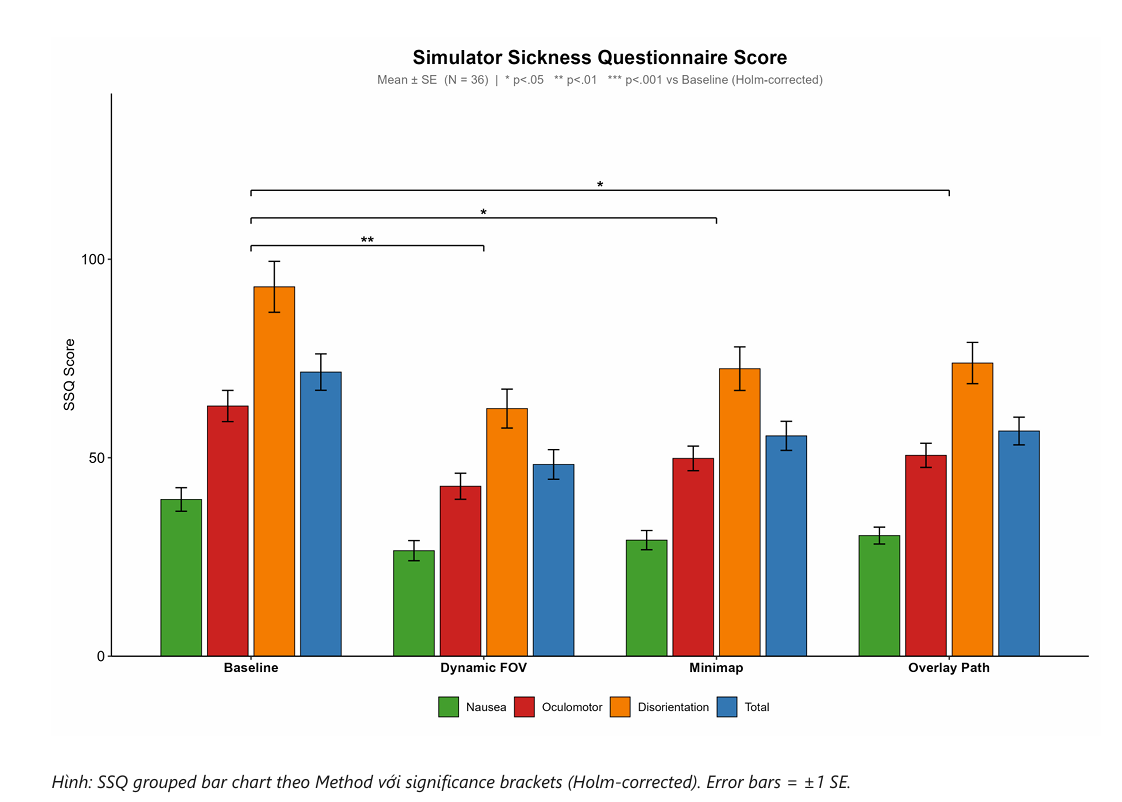
\includegraphics[width=0.88\textwidth]
        {figures/study1_ssq_by_method.png}
    }{}
    \caption{Simulator Sickness Questionnaire scores across visualization methods. Lower scores indicate less VIMS. Error bars show $\pm1$ SE; brackets indicate significant pairwise comparisons.}
    \label{fig:study1-ssq-method}
\end{figure*}


\subsubsection{Presence and the VIMS--Presence Trade-off}

The pattern for Presence differed from the SSQ results. Table~\ref{tab:study1-presence-pairwise} highlights the pairwise comparisons most relevant to the VIMS--Presence trade-off.

\begin{table}[t]
    \centering
    \caption{Key Bonferroni-adjusted pairwise comparisons for Presence.}
    \label{tab:study1-presence-pairwise}
    \small
    \begin{tabular}{lcc}
        \toprule
        \textbf{Comparison} & $\boldsymbol{\Delta}$ \textbf{Presence} & \textbf{$p$} \\
        \midrule
        Baseline -- Dynamic FOV & +0.861 & \textbf{.0006} \\
        Baseline -- Minimap & +0.254 & .1984 \\
        Baseline -- Overlay Path & +0.372 & \textbf{.0093} \\
        Dynamic FOV -- Minimap & -0.607 & \textbf{.0022} \\
        Dynamic FOV -- Overlay Path & -0.489 & \textbf{.0101} \\
        Minimap -- Overlay Path & +0.119 & 1.000 \\
        \bottomrule
    \end{tabular}
\end{table}

\paragraph{Dynamic FOV.}
Although Dynamic FOV achieved the largest numerical VIMS reduction, it also produced the \textbf{lowest Presence score} ($M=3.92$), significantly below the other three conditions.

\paragraph{Minimap.}
Minimap preserved Presence most effectively: its score did not significantly differ from Baseline ($p=.1984$).

\paragraph{Overlay Path.}
Overlay Path produced a smaller but significant reduction in Presence relative to Baseline ($p=.0093$).

These results indicate a clear \textbf{VIMS--Presence trade-off}: stronger sickness mitigation does not necessarily correspond to a better overall viewing experience.

% ------------------------------------------------------------
% FIGURE PLACEHOLDER: PRESENCE
% Export the Presence boxplot as:
% figures/study1_presence_by_method.png
% ------------------------------------------------------------

\begin{figure}[t]
    \centering
    \IfFileExists{figures/study1_presence_by_method.png}{
        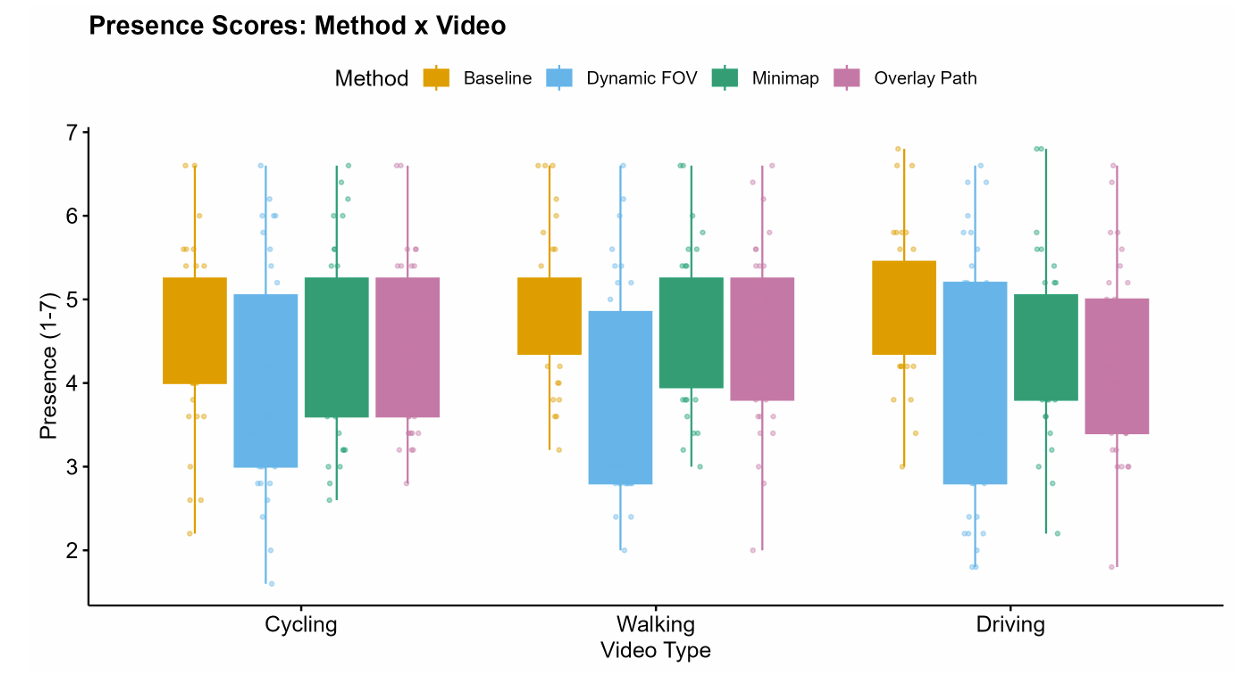
\includegraphics[width=\columnwidth]
        {figures/study1_presence_by_method.png}
    }{}
    \caption{Presence ratings across visualization methods and video types. Higher values indicate stronger perceived presence.}
    \label{fig:study1-presence}
\end{figure}


\subsubsection{Qualitative Feedback}

The interviews further explain the differences between the three mitigation methods. Table~\ref{tab:study1-mixed-methods} summarizes the main qualitative observations together with the corresponding quantitative results.

\begin{table*}[t]
    \centering
    \caption{Integration of quantitative and qualitative findings.}
    \label{tab:study1-mixed-methods}
    \small
    \begin{tabular}{
        p{0.14\textwidth}
        p{0.34\textwidth}
        p{0.44\textwidth}}
        \toprule

        \textbf{Method}
        & \textbf{Quantitative result}
        & \textbf{Interview feedback} \\

        \midrule

        Minimap
        &
        TSC reduced by 22\%; Presence remained closest to Baseline ($p=.1984$).
        &
        Familiar and stable for some participants, but its small size and low position required users to look away from the main scene, producing additional attention cost. \\

        Overlay Path
        &
        TSC reduced by 21\%; small Presence reduction relative to Baseline ($p=.0093$).
        &
        Helped some participants anticipate the camera trajectory. However, visual distraction and difficulty initially understanding the function of the path could interfere with the experience. \\

        Dynamic FOV
        &
        \textbf{Largest TSC reduction (33\%)}, but \textbf{lowest Presence} ($M=3.92$) and highest Presence variability ($SD=1.33$).
        &
        Highly polarized. Some participants reported that reducing peripheral motion helped alleviate discomfort, while others disliked the restricted peripheral view. \\

        \bottomrule
    \end{tabular}
\end{table*}

Overall, the interviews suggest that the effectiveness of each technique depends not only on sickness reduction, but also on how the visual aid affects attention, and even the exposure duration to the 360 video: \textbf{some participants even suggest that for longer 360 videos, they would trade immersion with VIMS reduction}. 


\subsubsection{Exploratory Preference Ranking}

Because preference rankings were available for only 13 of the 36 participants (36.1\%), these results are treated as exploratory. However in study 2, a complete reference ranking is available. 

\begin{table}[t]
    \centering
    \caption{Exploratory preference ranking. Lower mean rank indicates stronger preference. First- and last-choice counts are tie-adjusted.}
    \label{tab:study1-preference}
    \small
    \begin{tabular}{lcccc}
        \toprule
        \textbf{Method}
        & \textbf{Mean rank}
        & \textbf{Borda}
        & \textbf{First}
        & \textbf{Last} \\
        \midrule

        \textbf{Overlay Path} & \textbf{2.04} & \textbf{38.5} & 4.0 & \textbf{0.5} \\
        Minimap & 2.42 & 33.5 & 1.0 & 1.0 \\
        Dynamic FOV & 2.73 & 29.5 & \textbf{5.0} & \textbf{6.5} \\
        Baseline & 2.81 & 28.5 & 3.0 & 5.0 \\

        \bottomrule
    \end{tabular}
\end{table}

\paragraph{Overlay Path.}
Overlay Path had the \textbf{best overall mean rank and Borda score} and was almost never ranked last.

\paragraph{Dynamic FOV.}
Dynamic FOV again showed the strongest polarization: it received both the \textbf{largest number of first-choice rankings} and the \textbf{largest number of last-choice rankings}.

% OPTIONAL FIGURE
% figures/study1_preference_rank.png
%
% \begin{figure}[t]
%     \centering
%     \includegraphics[width=\columnwidth]
%     {figures/study1_preference_rank.png}
%     \caption{Mean preference rank across visualization methods.
%     Lower values indicate stronger preference.}
%     \label{fig:study1-preference-rank}
% \end{figure}


\subsubsection{Study 1 Summary}

Taken together, Study 1 shows that all three visualization techniques reduced VIMS relative to the unmodified Baseline, while their effects remained consistent across the three video types. \textbf{Dynamic FOV} provided the greatest numerical sickness reduction but substantially reduced Presence and produced polarized responses. \textbf{Minimap} provided the strongest quantitative balance between VIMS mitigation and Presence preservation. \textbf{Overlay Path} achieved a similar VIMS reduction while receiving the strongest exploratory preference ranking, although interview feedback highlighted the importance of clear and visually stable implementation.

